\documentclass[12pt, a4paper]{article}
\usepackage{ctex}
\usepackage{amsmath}
\usepackage{amsfonts}
\usepackage{amsthm}
\usepackage{ulem}
\usepackage{cancel}
\usepackage{graphicx}
\usepackage{theorem}
\usepackage{hyperref}
\usepackage[a4paper, left=2cm, top=2cm, total={170mm, 257mm}]{geometry}
\usepackage{color}
\usepackage{xcolor}
\usepackage{verbatim}
\usepackage{listings}
\lstset{
    basewidth=0.5em,
    frame=shadowbox, %用方框框住代码块
    numbers=left, %行号在左侧显示
    numberstyle=\tiny\ttfamily, %行号字体
    basicstyle=\small\ttfamily, %基本代码风格
    keywordstyle=\ttfamily\color{blue}, %关键字风格
    commentstyle=\ttfamily\itshape\color{red}, %注释风格
    stringstyle=\ttfamily\color{magenta}, %字符串风格
    rulesepcolor=\color{gray}, %代码块边框颜色
    backgroundcolor=\color{red!20!green!20!blue!20}, %代码块背景颜色
    breaklines=true, %代码过长则换行
    linewidth=0.9\linewidth,
    tabsize=4,
    columns=fixed,
    flexiblecolumns
}
\usepackage{fontspec}
\usepackage{caption}
\usepackage{float}

\setsansfont{Consolas}
\setmonofont{Fira Code}
\setCJKmainfont{Sarasa UI SC}
\setCJKsansfont{Sarasa Term SC}
\setCJKmonofont{Sarasa Mono SC}

\title{吴恩达机器学习读书笔记 \\ Machine Learning by Andrew Ng}
\author{Zhaorui.Zhan}
\date{}
\begin{document}
\maketitle

\begin{abstract}    
    基于吴恩达在Coursera上的公开课Machine Learning做的笔记。对定性部分进行了一些省略,重点关注算法的使用与逻辑推导。
\end{abstract}

\tableofcontents
\newpage

\section{引言 Introduction}

监督学习是给学习算法的一个数据集中,数据集样本本身已经提供了“正确答案”,需要根据这些样本做出预测。而无监督学习中,数据集没有任何标签,需要算法根据数据集本身对其进行分类或标记,从而找出某种结构。

针对连续值的预测称为回归问题,对于离散值的预测称为分类问题。

\section{单变量线性回归 Linear Regression with One Variable}

\subsection{模型表示}

对于回归问题的标记,通常定义为:

\begin{enumerate}
    \item 
          $m$:训练集中实例的数量(有多少个样本)
    \item 
          $y$:特征/输入变量
    \item 
          $(x, y)$:目标变量/输出变量
    \item 
          $(x^{(i)}, y^{(i)})$:第$i$个观测实例
    \item 
          $h$:学习算法的函数,也称为假设\textit{hypothesis}
\end{enumerate}

最简单的预测方式为$h_\theta(x)=\theta_0 + \theta_1x$,因为只含有一个特征变量,因此这种问题被称为单变量线性回归问题。

\subsection{代价函数}

当已经创建了假设函数,即用来预测的函数形式为:$h_\theta(x)=\theta_0 + \theta_1x$,后续的问题是如何对使用的模型选择合适的参数$\theta_i$。在单变量线性回归中,需要选择的就是直线的斜率$\theta_1$和截距项$\theta_0$。

由于选择的参数决定了得到的模型对应的直线相对于训练集的准确程度,模型所预测的值与训练集中实际值的差异就是建模误差\textit{modelling error},即$y_i - \hat{y}_i$。

选择参数的过程就是选择将建模误差的平方和最小的参数。

在这里定义代价函数$J(\theta_0, \theta_1)$,当$J(\theta_0, \theta_1)$最小时,选择的参数为最优参数。即:

\begin{align*}
     & \mathbf{Hypothesis}: h_\theta(x)=\theta_0 + \theta_1x                                                   \\
     & \mathbf{Cost Function}: J(\theta_0, \theta_1) = \frac{1}{2m}\sum_{i=1}^{m}(h_\theta(x^{(i)})-y^{(i)})^2 \\
     & \mathbf{Goal}: \mathop{minimize}\limits_{\theta_0, \theta_1}J(\theta_0, \theta_1)
\end{align*}

对上述代价函数进行简化,假设$\theta_0=0$,同时只有三个样本点$(1,1),(2,2),(3,3)$:

对于这个简化的模型,可以选择无数个$\theta_1$进行模拟:

\begin{enumerate}
    \item 
          $\theta_1=0$
          
          \begin{align*}
               & h_\theta(x) = 0                                     \\
               & J(0) = \frac{1}{2*3}(-1^2+-2^2+-3^2) = \frac{14}{6}
          \end{align*}
          
    \item 
          $\theta_1=0.5$
          
          \begin{align*}
               & h_\theta(x) = 0.5x                                       \\
               & J(0) = \frac{1}{2*3}(-0.5^2+-1^2+-1.5^2) = \frac{3.5}{6}
          \end{align*}
          
    \item 
          $\theta_1=1$
          
          \begin{align*}
               & h_\theta(x) = x                       \\
               & J(0) = \frac{1}{2*3}(0^2+0^2+0^2) = 0
          \end{align*}
          
    \item 
          $\dots$
\end{enumerate}

\begin{figure}[H]
    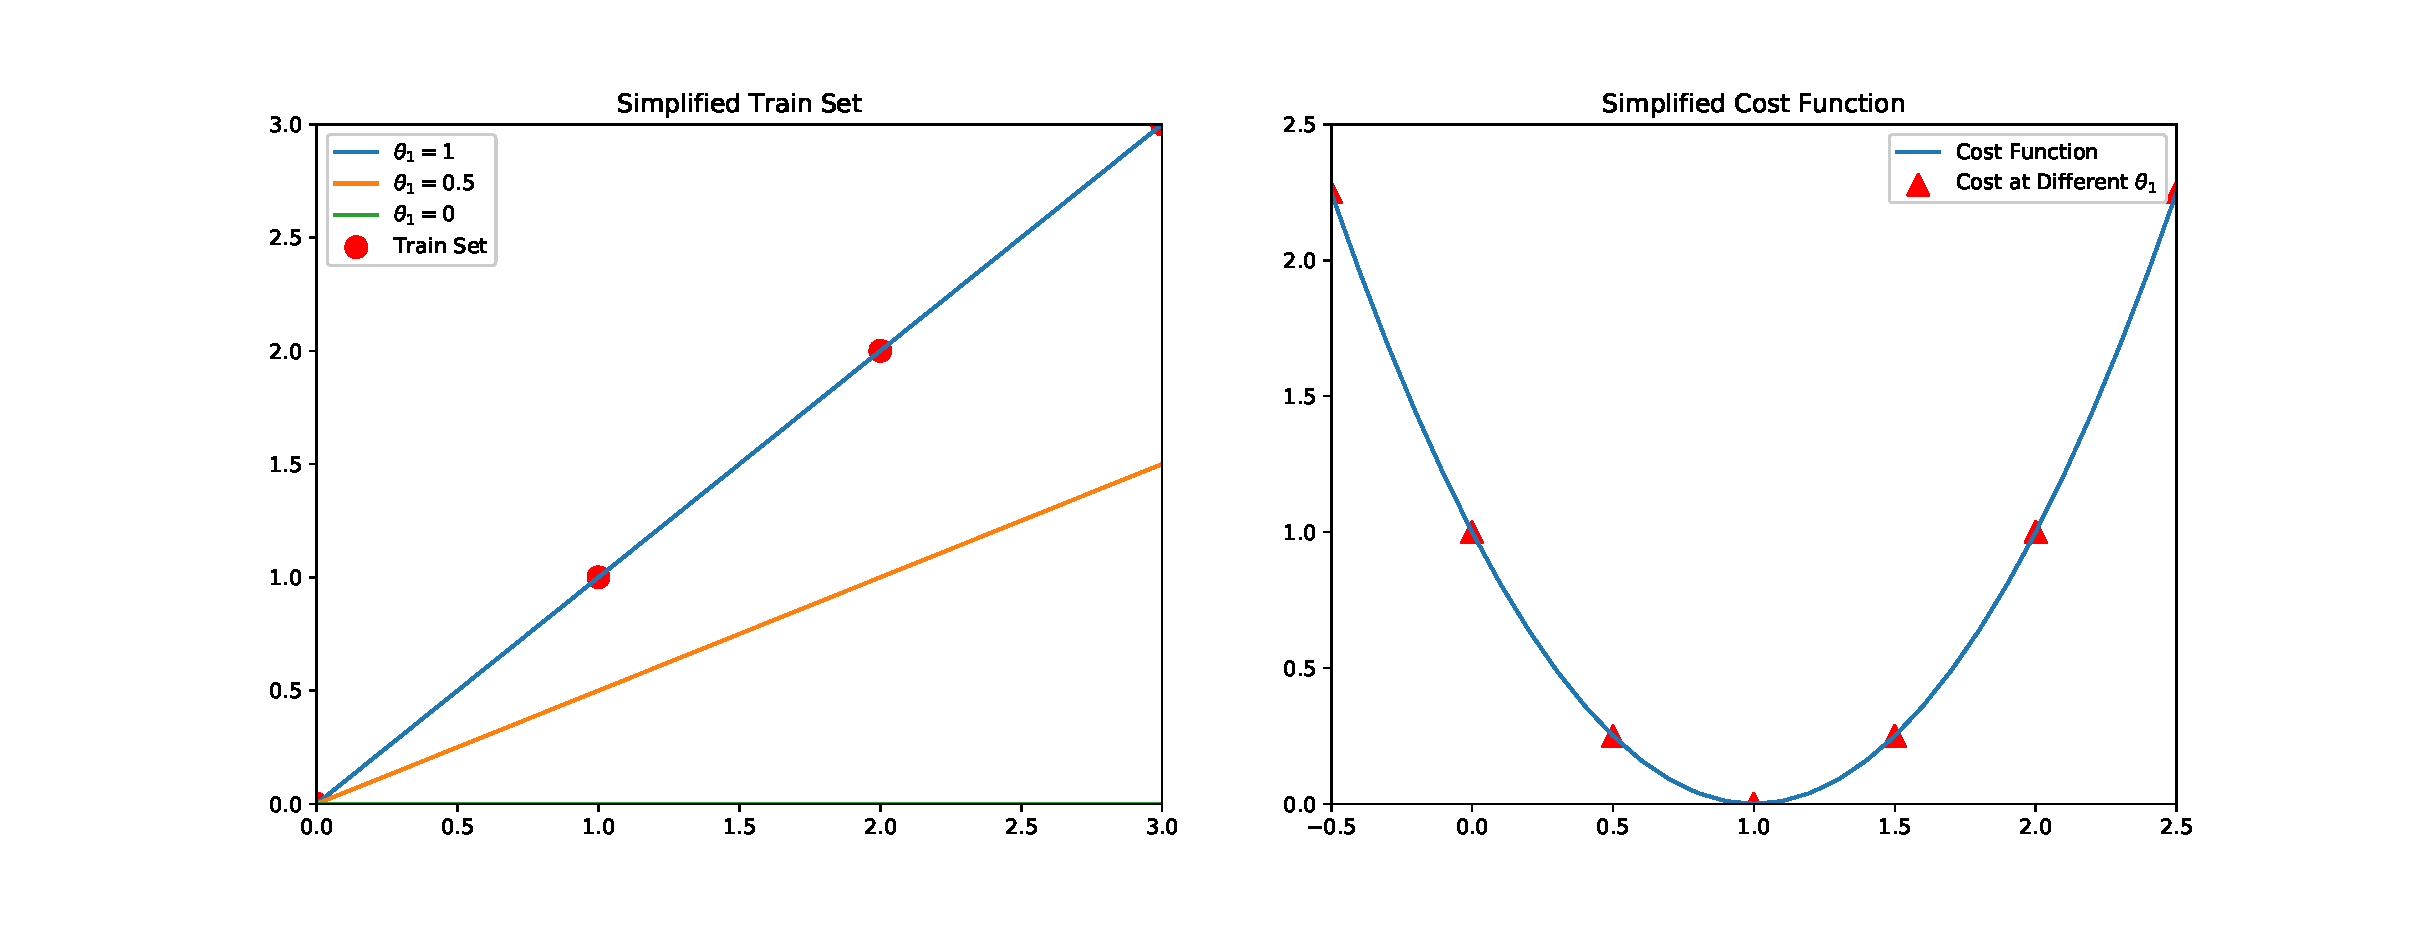
\includegraphics[width=1\textwidth]{OneParameterCostFunction.eps}
\end{figure}

将这些点连在一起形成的曲线,就构成了一个参数下的代价函数曲线。实际上,将三个样本点带入后,可以得到这里的代价函数$J(\theta_1)$的解析式为$J(\theta_1)=\frac{14}{6}(\theta_1-1)^2$。

在课程中,展示了非常漂亮的等高线图及使用梯度下降法找到最优$\theta_0, \theta_1$的图像,但是通过实际测试,并不能画出类似的图像,此处是是否是个人理解出现问题存疑,将代码和对应的图片放在这里作为后续参考:

\begin{lstlisting}[language=Python]
import numpy as np
import matplotlib.pyplot as plt
from mpl_toolkits.mplot3d import Axes3D

x = np.arange(0, 10, 0.05)
y = x + np.random.rand(len(x)) * 2

reg = linear_model.LinearRegression()
reg.fit(x.reshape(-1, 1), y)

theta0 = theta1 = np.linspace(-2.5, 4)
theta0, theta1 = np.meshgrid(theta0, theta1)
err = 0.0
for i in range(len(x)):
    err += np.power((theta0 + theta1 * x[i] - y[i]), 2)
err = err / (2 * len(x))

plt.figure(figsize=(18, 6))
ax1 = plt.subplot(121)
ax1.scatter(x, y)
ax1.plot(x, reg.predict(x.reshape(-1, 1)), color='r')
ax1.set_title('Linear Regression')

ax2 = plt.subplot(122, projection='3d')
ax2.plot_surface(theta0, theta1, err, cmap='rainbow')
ax2.contour(theta0, theta1, err, zdir='r', offset=-2)
ax2.set_title('Cost Function')
           \end{lstlisting}

\begin{figure}[H]
    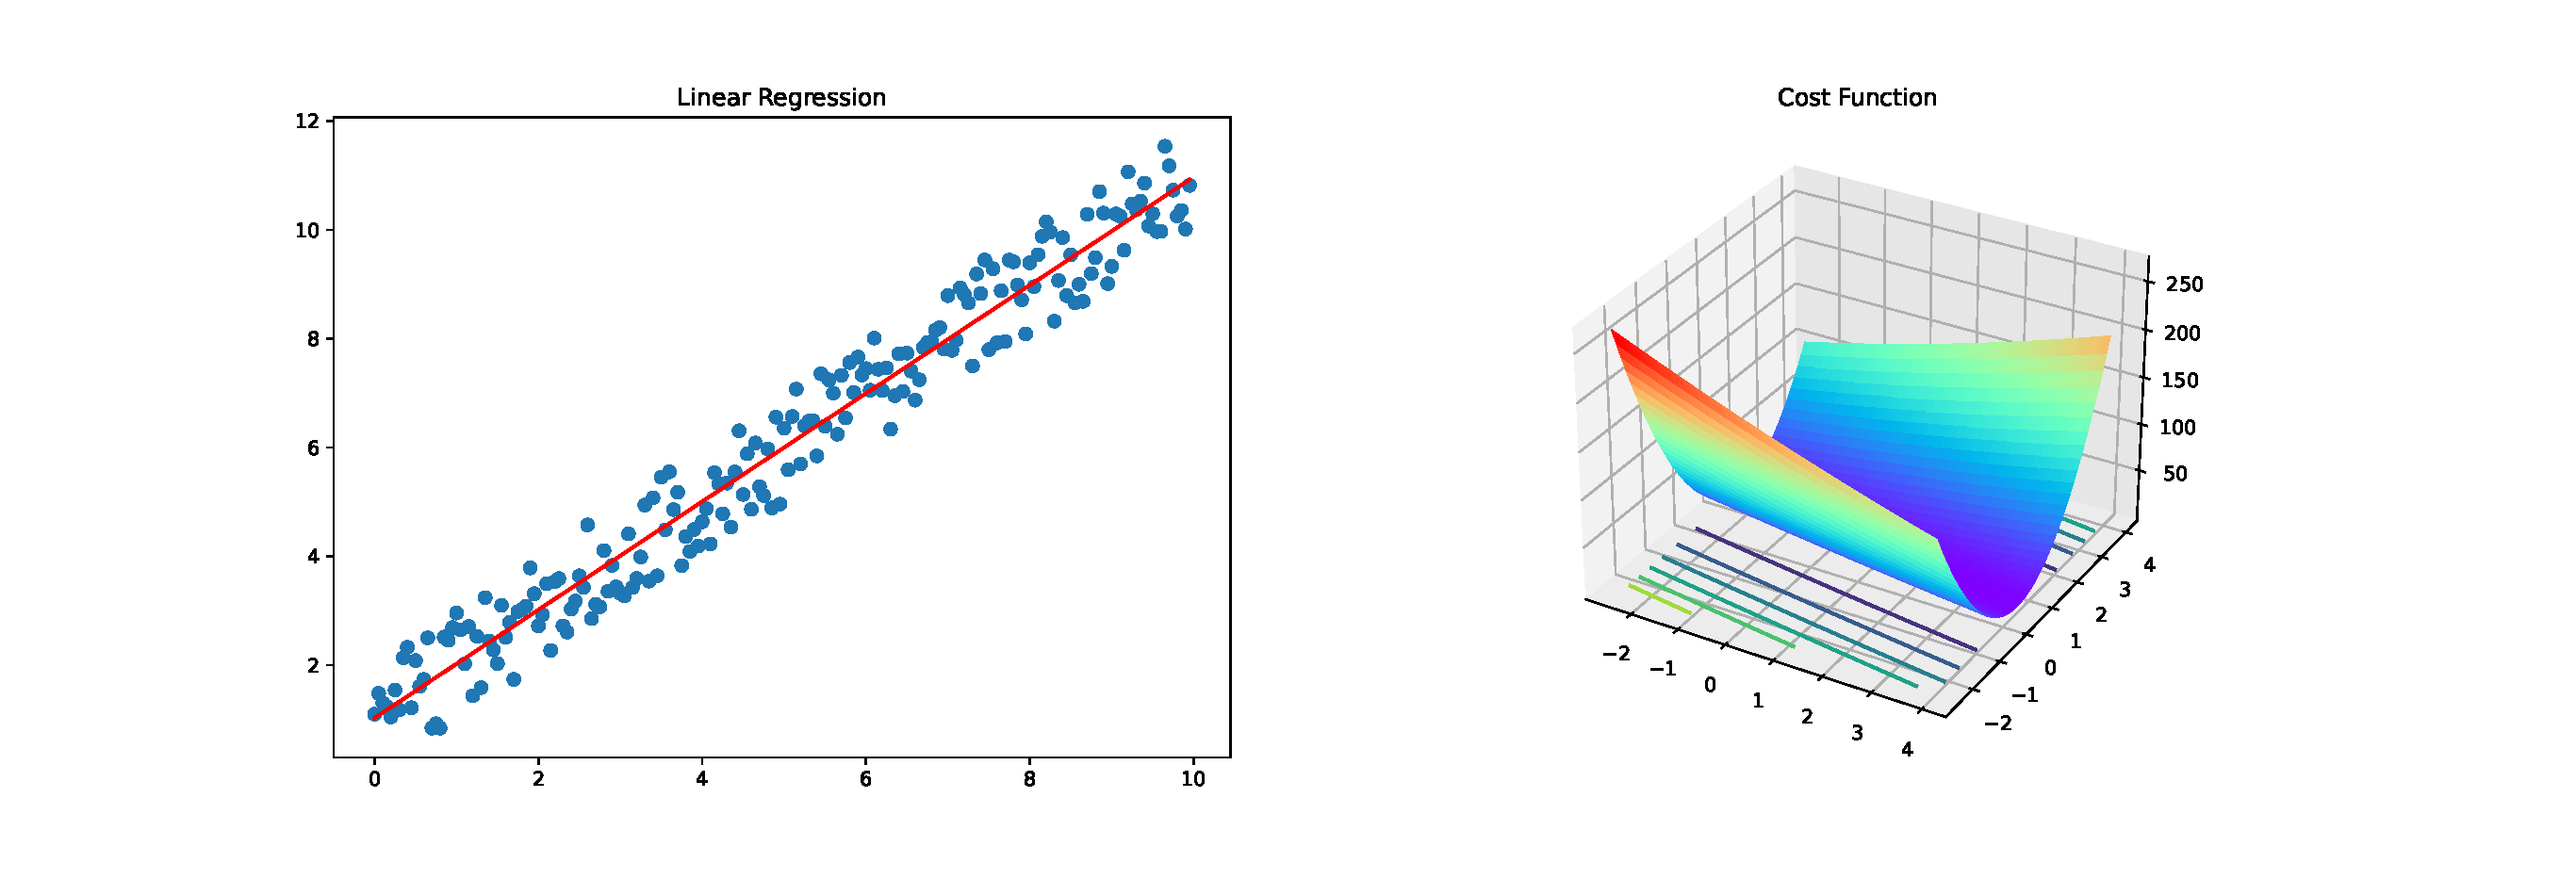
\includegraphics[width=1\textwidth]{CostFunction.eps}
\end{figure}

\subsection{梯度下降}

当有了代价函数$J$之后,就需要找到使代价函数$J$最小的$\theta_0, \theta_1$。梯度下降法就是一种非常好的用来求函数最小值的算法。其本质是每次迭代中找出函数在当前参数下下降最快的方向,然后逐步迭代找到局部最小值。当需要优化的函数是一个凸函数时,局部最小值也是全局最小值。此外,梯度下降要求给出一个学习速率(learning rate)$\alpha$,这对应着每次迭代时所移动的步长。

这里使用的梯度下降算法为批梯度下降(batch gradient descent),即在每次迭代中必须要同时更新所有需要优化的参数,让所有的参数减去学习速率乘以代价函数的导数,然后才能进行下一次迭代。

批量梯度下降算法为:

\begin{equation*}
    \theta_j:=\theta_j-\alpha\frac{\partial}{\partial\theta_j}J(\theta)
\end{equation*}

在梯度下降算法中,学习速率的选择需要一些技巧。如果学习速率选择的过小,则算法收敛至局部最小值所消耗的时间过长,而如果学习速率选择的过大,则可能会导致迭代越过最低点,从而无法找到局部最小值甚至导致算法结果从收敛转向发散。

回到前面两个参数的线性回归问题中,对于线性回归问题使用梯度下降法,关键在于求出代价函数的导数,即:

\begin{align*}
    \frac{\partial}{\partial\theta_j}J(\theta)                                & =\frac{\partial}{\partial\theta_j}\frac{1}{2m}\sum_{i=1}^{n}(h_\theta(x^{(i)})-y^{(i)})^2 \\
    \text{if}\ j=0:\quad\frac{\partial}{\partial\theta_0}J(\theta_0,\theta_1) & =\frac{1}{m}\sum_{i=1}^{m}(h_\theta(x^{(i)})-y^{(i)})                                     \\
                                                                              & =\frac{1}{m}\sum_{i=1}^{m}(\theta_0+\theta_1x_i-y_i)                                      \\
    \text{if}\ j=1:\quad\frac{\partial}{\partial\theta_1}J(\theta_0,\theta_1) & =\frac{1}{m}\sum_{i=1}^{m}((h_\theta(x^{(i)})-y^{(i)})\cdot x^{(i)})                      \\
                                                                              & =\frac{1}{m}\sum_{i=1}^{m}((\theta_0+\theta_1x_i-y_i)\cdot x_i)
\end{align*}

从而:

\begin{align*}
    \theta_0 & :=\theta_0-\alpha\frac{1}{m}\sum_{i=1}^{m}(\theta_0+\theta_1x_i-y_i)            \\
    \theta_1 & :=\theta_1-\alpha\frac{1}{m}\sum_{i=1}^{m}((\theta_0+\theta_1x_i-y_i)\cdot x_i)
\end{align*}

仍然使用之前的示例,尝试进行线性回归并验算结果:

\begin{enumerate}
    \item 
          首先导入必要的Python库并构造数据集:
          
          \begin{lstlisting}[language=Python]
import numpy as np
# 指定使用的随机数种子
np.random.seed(0)

# 创建模拟数据
x = np.arange(0, 10, 0.05)
y = x + np.random.rand(len(x)) * 2
               \end{lstlisting}
          
    \item 
          进行梯度下降算法:
          
          使用矩阵计算代价函数对于参数$\theta$的偏导:
          
          \begin{align*}
              \theta_j & :=\theta_j-\alpha\frac{\partial}{\partial\theta_j}J(\theta)                                         \\
              \theta_j & :=\theta_j-\alpha\frac{\partial}{\partial\theta_j}(\frac{1}{2m}\sum_{i=1}^{m}(h_\theta(x^i)-y^i))^2 \\
              \theta_j & :=\theta_j-\frac{\alpha}{m}\sum_{i=1}^{m}(\theta_0x_0^i+\theta_1x_1^i+\dots-y^i)\cdot x_j^i
          \end{align*}
          
          对于一个$(m\times j)$的矩阵$X$,$m$为样本数量,$j$为特征$x$的数量,有对应的系数为$(1\times j)$的矩阵$\Theta$及$(m\times 1)$的因变量矩阵$Y$,可以将代价函数的导数部分化简为:
          
          \begin{align*}
              X \times \Theta^T & = 
              \left[
                  \begin{matrix}
                      x_0^1  & x_1^1  & \cdots & x_j^1  \\
                      x_0^2  & x_1^2  & \cdots & x_j^2  \\
                      \vdots & \vdots & \ddots & \vdots \\
                      x_0^m  & x_1^m  & \cdots & x_j^m
                  \end{matrix}
                  \right]
              \left[
                  \begin{matrix}
                      \theta_0 \\
                      \theta_1 \\
                      \cdots   \\
                      \theta_j  
                  \end{matrix}
                  \right]            \\
                                & = 
              \left[
                  \begin{matrix}
                      \theta_0x_0^1+\theta_1x_1^1+\dots+\theta_jx_j^1 \\
                      \vdots                                          \\
                      \theta_0x_0^m+\theta_1x_1^m+\dots+\theta_jx_j^m \\
                  \end{matrix}
                  \right]
          \end{align*}
          
          因此:
          
          \begin{align*}
                & \left[
                  \begin{matrix}
                       & \sum_{i=1}^{m}(\theta_0x_0^i+\theta_1x_1^i+\dots+\theta_jx_j^i-y^i)\cdot x_0^i \\
                       & \vdots                                                                         \\
                       & \sum_{i=1}^{m}(\theta_0x_0^i+\theta_1x_1^i+\dots+\theta_jx_j^i-y^i)\cdot x_j^i \\
                  \end{matrix}
                  \right] \\
              = & 
              \left[
                  \begin{matrix}
                      x_0^1  & \cdots & x_0^m  \\
                      \vdots & \ddots & \vdots \\
                      x_j^1  & \cdots & x_j^m
                  \end{matrix}
                  \right]
              \left(\left[
                  \begin{matrix}
                      \theta_0x_0^1+\theta_1x_1^1+\dots+\theta_jx_j^1 \\
                      \vdots                                          \\
                      \theta_0x_0^m+\theta_1x_1^m+\dots+\theta_jx_j^m \\
                  \end{matrix}
                  \right]-
              \left[
                  \begin{matrix}
                      y^1    \\
                      \vdots \\
                      y^m
                  \end{matrix}
                  \right]\right)
          \end{align*}
          
          即:
          
          \begin{align*}
              \theta_j          & :=\theta_j-\frac{\alpha}{m}\sum_{i=1}^{m}(\theta_0x_0^i+\theta_1x_1^i+\dots-y^i)\cdot x_j^i \\
              \Rightarrow\Theta & :=\Theta-\frac{\alpha}{m}X^T(X\times \Theta^T-Y)
          \end{align*}
          
          当只有两个参数$\theta_0,\theta_1$时,由于$\theta_0$对应的是截距项,因此可以对$x$增加全为1的列作为$x_0$,使其可以进行矩阵运算,同时设定学习速率$\alpha$和初始点:
          
          \begin{lstlisting}[language=Python]
X = np.stack((np.ones(len(x)), x), axis=1)
Y = y
# 设定学习速率
alpha = 0.01
# 设定初始点
theta = np.array([0.0, 0.0])
gradient = alpha / len(y) * (X.T.dot(X.dot(theta.T) - Y))
# 计算代价函数
cost = np.sum(np.power(X.dot(theta.T) - Y, 2)) / (2 * len(y))
costs = [cost]
while not (np.isclose(gradient[0], 0) and np.isclose(gradient[1], 0)):
    theta = theta - gradient
    gradient = alpha / len(y) * (X.T.dot(X.dot(theta.T) - Y))
    cost = np.sum(np.power(X.dot(theta.T) - Y, 2)) / (2 * len(y))
    costs.append(cost)
print("Iteration: {}, theta_0={:.4f}, theta_1={:.4f}".format(len(costs), theta[0], theta[1]))
# Iteration: 4974, theta_0=1.0283, theta_1=0.9945
               \end{lstlisting}
          
          在迭代4974次后$\theta$变化量约等于0,迭代结束,得到计算出的$\theta$值。
          
    \item 
          使用scikit-learn进行线性回归,校验梯度下降得出的结果:
          
          \begin{lstlisting}[language=Python]
from sklearn import linear_model
reg = linear_model.LinearRegression()
reg.fit(x.reshape(-1, 1), y)
print("theta_0={:.4f}, theta_1={:.4f}".format(reg.intercept_, reg.coef_[0])))
# theta_0=1.0283, theta_1=0.9945
               \end{lstlisting}
          
          结果一致。
\end{enumerate}

\section{线性代数回顾 Linear Algebra Review}

\begin{enumerate}
    \item 
          矩阵乘法不服从交换律:$A\times B\neq B\times A$。
    \item 
          矩阵乘法服从结合律:$A\times(B\times C) = (A\times B)\times C$。
    \item 
          单位矩阵$I$类似于数乘中的1,$I$是一个方阵,满足$AA^{-1}=A^{-1}A=I$。对于任意矩阵,$AI=IA=A$,这里两个单位矩阵的维度不一定是相同的,其维度隐含在$A$的维度中。
    \item 
          只有方阵才有逆矩阵,但不是所有方阵都有逆矩阵。没有逆矩阵的矩阵称为奇异矩阵。
    \item 
          矩阵转置的基本性质:
          
          \begin{align*}
               & (A\pm B)^T = A^T\pm B^T       \\
               & (A\times B)^T = B^T\times A^T \\
               & (A^T)^T = A                   \\
               & (KA)^T = KA^T
          \end{align*}
\end{enumerate}

\section{多元线性回归 Linear Regression with Multiple Variables}

在单变量线性回归中,

\begin{equation*}
    h_\theta(x) = \theta_0 + \theta_1x_1
\end{equation*}

在多元线性回归中,$h_\theta(x)$将拓展为:

\begin{equation*}
    h_\theta(x)=\theta_0 + \theta_1x_1+ \theta_2x_2+\cdots+\theta_nx_n
\end{equation*}

同样,为了便于使用矩阵形式表述,定义$x_0=1$,因此,

\begin{equation*}
    h_\theta(x)=\theta_0x_0 + \theta_1x_1+ \theta_2x_2+\cdots+\theta_nx_n
\end{equation*}

在这里:

\begin{equation*}
    X=\left[
        \begin{matrix}
            x_0    \\
            x_1    \\
            \vdots \\
            x_n
        \end{matrix}
        \right]\in\mathbb{R}^{n+1}\quad
    \Theta=\left[
        \begin{matrix}
            \theta_0 \\
            \theta_1 \\
            \vdots   \\
            \theta_n
        \end{matrix}
        \right]\in\mathbb{R}^{n+1}
\end{equation*}

从而有:

\begin{align*}
    h_\theta(x) & =\theta_0x_0 + \theta_1x_1+ \theta_2x_2+\cdots+\theta_nx_n \\
                & =\Theta^TX
\end{align*}

和单变量线性回归一样,这里给出多元线性回归的模型表示:

\begin{align*}
     & \mathbf{Hypothesis}: h_\theta(x)=\Theta^TX=\theta_0x_0 + \theta_1x_1 + \theta_2x_2+\cdots+\theta_nx_n                          \\
     & \mathbf{Parameters}:\Theta=\theta_0,\theta_1,\dots,\theta_n                                                                    \\
     & \mathbf{Cost Function}:J(\Theta)=J(\theta_0,\theta_1,\dots,\theta_n) = \frac{1}{2m}\sum_{i=1}^{m}(h_\theta(x^{(i)})-y^{(i)})^2 \\
     & \mathbf{Goal}: \mathop{minimize}\limits_{\Theta}J(\Theta)
\end{align*}

批量梯度下降算法同样为(注意对每个$j=0,\dots,n$要同步更新$\theta$):

\begin{equation*}
    \theta_j:=\theta_j-\alpha\frac{\partial}{\partial\theta_j}J(\Theta)
\end{equation*}

\section{逻辑回归 Logistic Regression}

\section{正则化 Regularization}

\section{神经网络:表述 Neural Networks: Representation}

\section{神经网络:学习 Neural Networks: Learning}

\section{应用机器学习的建议 Advice for Apply Machine Learning}

\section{机器学习系统的设计 Machine Learning System Design}

\section{支持向量机 Support Vector Machines}

\section{聚类 Clustering}

\section{降维 Dimensionality Reduction}

\section{异常检测 Anomaly Detection}

\section{推荐系统 Recommender Systems}

\section{大规模机器学习 Large Scale Machine Learning}

\section{结语 Conclusion}

\end{document}